%% Karlsruhe Institute of Technology
%% Institute for Anthropomatics and Robotics (IAR)
%% Artificial Intelligence for Language Technologies (AI4LT) lab
%%
%% Prof. Dr. Jan Niehues
%% Lab's website https://ai4lt.anthropomatik.kit.edu/english/index.php

\iflanguage{english}
{\chapter{Appendix}}    % english style
{\chapter{Anhang}}      % german style
\label{chap:appendix}


%% -------------------
%% | Example content |
%% -------------------

\section{Other interesting pearson correlation scores}\label{dropout softmax entropy}

The pearson correlation of the entropies in dropout shows a significant prediction value with a correlation of the mean of -0.23241 and 0.29450, and a correlation of -0.17032 and - 0.12806 of the variance of the entropies on seamless and deltaLM respectively. Which is higher than just the regular translation probability and variance but it comes with a significant cost to compute as calculating the softmax entropy is very rarely implemented in frameworks.
\section{references graphs}
\label{sec:appendix:FirstSection}
Since there are a lot of plots that contain plots over the reference scores it might be intersting to see how those references fall over the data set. 

\setcounter{figure}{0}

\begin{figure}[ht]
    \centering
    \begin{subfigure}{0.7\textwidth}
    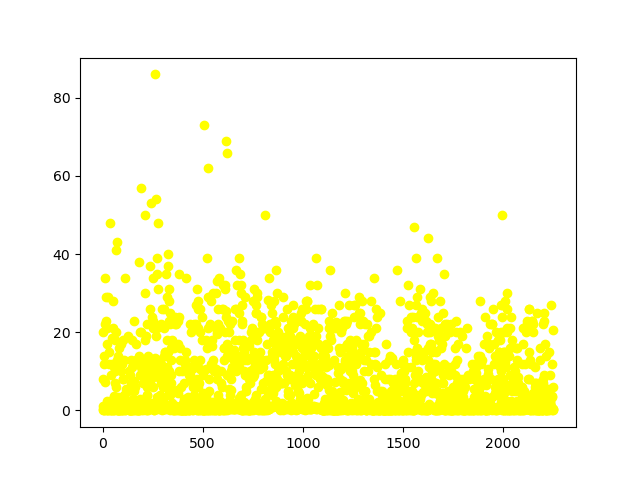
\includegraphics[width=\linewidth]{Latex/sections/images/seamlesswerref.png}
    \caption{all of the reference scores of the dataset, the x axis is the lines in teh dataset, the y axis is the WER scores}
    \end{subfigure}
    \begin{subfigure}{0.7\textwidth}
        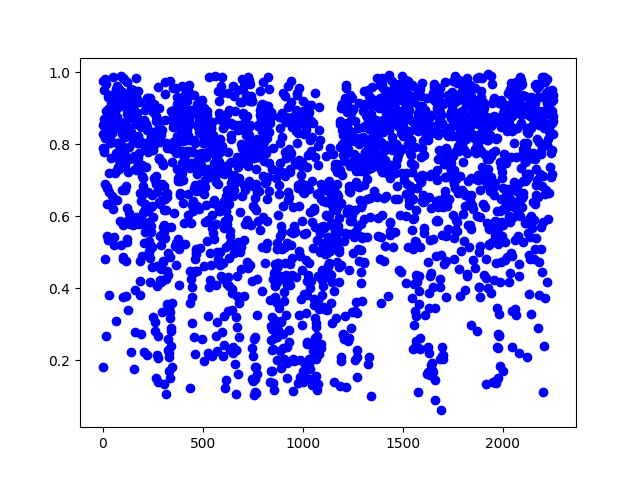
\includegraphics[width=\linewidth]{Latex/sections/images/seamlessreferences.png}
        \caption{refrence coment scores from seamless}
    \end{subfigure}
    \label{fig:reference scatterplot}
\end{figure}



%% ---------------------
%% | / Example content |
%% ---------------------